\chapter{Relations Among Variables: Advanced}
\label{chap:advrels}

\section{Nonlinear Parametric Regression Models}
\label{nonlin}

We pointed out in Section \ref{whatmeans} that the word {\it linear} in
{\it linear regression model} means linear in $\beta$, not in t.  This
is the most popular approach, as it is computationally easy, but
nonlinear models are often used.

The most famous of these is the {\bf logistic} model, for the case in
which $Y$ takes on only the values 0 and 1.  As we have seen before
(Section \ref{indicator}), in this case the expected value becomes a
probability.  The logistic model for a nonvector $X$ is then

\begin{equation}
\label{logit}
m_{Y;X}(t) = P(Y = 1 | X = t) = \frac{1}{1+e^{-(\beta_0+\beta_1 t})}
\end{equation}

It extends to the case of vector-valued $X$ in the obvious way. 

The logistic model is quite widely used in computer science, in medicine,
economics, psychology and so on.  We'll return to this model in Section
\ref{logitsec}.

Here is an example of a nonlinear model used in kinetics of chemical
reactions, with r = 3: \footnote{See
\url{http://www.mathworks.com/access/helpdesk/help/toolbox/stats/rsmdemo.html}.}

\begin{equation}
m_{Y;X}(t) = \frac
{\beta_1 t^{(2)} - t^{(3)}/\beta_5}
{1+\beta_2 t^{(1)} + \beta_3 t^{(2)} + \beta_4 t^{(3)}}
\end{equation}

Here the X vector is (hydrogen, n-pentane, isopentane) and Y is the
reaction rate.

Unfortunately, in most cases, the least-squares estimates of the
parameters in nonlinear regression do not have closed-form solutions,
and numerical methods must be used.  But R does that for you, via the
{\bf nls()} function in general, and via {\bf glm()} for the logistic
and related models in particular.

\section{The Classification Problem}
\label{class}

As mentioned earlier, in the special case in which Y is an indicator
variable, with the value 1 if the object is in a class and 0 if not, the
regression problem is called the {\bf classification problem}.  
If there are c classes, we need c (or c-1) Y variables, which I will 
denote by $Y^{(i)}$, i = 1,...,c.

Here are some examples:

\begin{itemize}

\item A forest fire is now in progress.  Will the fire reach a certain
populated neighborhood?  Here Y would be 1 if the fire reaches the
neighborhood, 0 otherwise.  The predictors might be wind direction,
distance of the fire from the neighborhood, air temperature and
humidity, and so on.

\item Is a patient likely to develop diabetes?  This problem has been
studied by many researchers, e.g.  Using Neural Networks To Predict the
Onset of Diabetes Mellitus, Murali S. Shanker {\it J. Chem. Inf. Comput.
Sci.}, 1996, 36 (1), pp 35–41.  A famous data set involves Pima Indian
women, with Y being 1 or 0, depending on whether the patient does
ultimately develop diabetes, and the predictors being the number of
times pregnant, plasma glucose concentration, diastolic blood pressure,
triceps skin fold thickness, serum insulin level, body mass index,
diabetes pedigree function and age. 

\item Is a disk drive likely to fail soon?  This has been studied for
example in Machine Learning Methods for Predicting Failures in Hard
Drives: A Multiple-Instance Application, by Joseph F. Murray, Gordon F.
Hughes, and Kenneth Kreutz-Delgado, {\it Journal of Machine Learning
Research} 6 (2005) 783-816.  Y was 1 or 0, depending on whether the
drive failed, and the predictors were temperature, number of read
errors, and so on.

\end{itemize}

In electrical engineering the classification is called {\bf pattern
recognition}, and the predictors are called {\bf features}.  In computer
science the term {\bf machine learning} usually refers to classification
problems.  Different terms, same concept.

\subsection{Classification = Regression}
\label{meanisprob}

{\it Do onto others as you would have them do onto you; all the rest is
commentary}---ancient Jewish philosopher Hillel, describing the Talmud

The above quote is not about who first stated the Golden Rule---it has
been found to be universal in religions and philosophies---but rather
that Hillel pointed out that the entire Talmud really boils down to one
simple idea.

Similarly, all of the many machine learning algorithms, despite their
complexity, really boil down to regression at their core.  Here's why:

As we have frequently noted the mean of any indicator random variable is
the probability that the variable is equal to 1 (Section
\ref{indicator}).  Thus in the case in which our response variable Y
takes on only the values 0 and 1, i.e.  classification problems, the
regression function reduces to

\begin{equation}
m_{Y;X}(t) = P(Y = 1 | X = t)
\end{equation}

(Remember that X and t are vector-valued.)

As a simple but handy example, suppose Y is gender (1 for male, 0 for
female), $X^{(1)}$ is height and $X^{(2)}$ is weight, i.e. we are
predicting a person's gender from the person's height and weight.  Then
for example, $m_{Y;X}(70,150)$ is the probability that a person of
height 70 inches and weight 150 pounds is a man.  Note again that this
probability is a population fraction, the fraction of men among all
people of height 70 and weight 150 in our population.

Make a mental note of the optimal prediction rule, if we know the
population regression function:

\begin{quote}
Given X = t, the optimal prediction rule is to predict that Y = 1 if and
only if $m_{Y;X}(t) > 0.5$.
\end{quote}

So, if we known a certain person is of height 70 and weight 150, our
best guess for the person's gender is to predict the person is male
if and only if $m_{Y;X}(70,150) > 0.5$.

The optimality makes intuitive sense, and is shown in the next section
\ref{optimal2}. 

\subsection{Optimality of the Regression Function for 0-1-Valued Y
(optional section)}
\label{optimal2}

Remember, our context is that we want to guess Y, knowing X.  Since Y is
0-1 valued, our guess for Y based on X, g(X), should be 0-1 valued too.
What is the best function g()?

Again, since Y and g are 0-1 valued, our criterion should be what will I
call Probability of Correct Classification (PCC):\footnote{This assumes
equal costs for the two kinds of classification errors, i.e. that
guessing Y = 1 when Y = 0 is no more or no less serious than the
opposite error.}

\begin{equation}
\label{pcc}
\textrm{PCC} = P[Y = g(X)]
\end{equation}

We'll show intuitively that the best rule, i.e. the g() that maximizes
(\ref{pcc}), is given by the function

\begin{equation}
g(t) = 
\begin{cases}
0, \textrm{ if } g(t) \leq 0.5 \cr
1, \textrm{ if } g(t) > 0.5 \cr
\end{cases}
\end{equation}

Think of this:  There is a biased coin, with known probability of heads
p.  The coin will be tossed once, and you are supposed to guess the
outcome.  

Let's formalize that.  Name your guess q, and let C denote the outcome
of the toss (1 for heads, 0 for tails).  Then the probability that you
guess correctly is

\begin{eqnarray}
P(C = q) &=& P(C = 1) q + P(C = 0) (1-q) \\ 
&=& P(C = 1) q + [1 - P(C = 1)] (1-q) \\ 
&=& [2 P(C = 1) - 1] q + 1 - P(C = 1) 
\end{eqnarray}

(That first equation merely accounts for the two cases, q = 1 and q =
0.  For example, if you choose q = 0, then the right-hand side reduces
to P(C = 0), as it should.)

Inspecting the last of the three equations above, we see that if P(C =
1) $>$ 0.5, then [2 P(C = 1) - 1 is positive, and thus q = 1 gives us a
larger P(C = q) value than does q = 0.  The reverse is true in the
nonpositive case.

To finish the proof, we would take P(C = q) above as the conditional
probability P(Y = g(X) $|$ X), and then apply an ``outer'' expected
value, using the material in Section \ref{lte}.

\subsection{Logistic Regression:  a Common Parametric Model for the
Regression Function in Classification Problems}
\label{logitsec}

Remember, we often try a parametric model for our regression function
first, as it means we are estimating a finite number of quantities,
instead of an infinite number.  Probably the most commonly-used model is
that of the logistic function (often called ``logit''), introduced in
Section \ref{nonlin}.  Its r-predictor form is 

\begin{equation}
\label{logit2}
m_{Y;X}(t) = P(Y = 1 | X = t) = \frac{1}{1+e^{-(\beta_0+\beta_1
t_1+...+\beta_r t_r)}}
\end{equation}

For instance, consider the patent example in Section \ref{examples}.
Under the logistic model, the population proportion of all patents that
are publicly funded, among those that contain the word ``NSF,'' do not
contain ``NIH,'' and make five claims would have the value

\begin{equation}
\frac{1}{1+e^{-(\beta_0 + \beta_1 + 5\beta_3)}}
\end{equation}

\subsubsection{The Logistic Model:  Motivations}
\label{logitmotivations}

The logistic function itself, 

\begin{equation}
\frac{1}{1+e^{-u}}
\end{equation}

has values between 0 and 1, and is thus a candidate for modeling a
probability.  Also, it is monotonic in u, making it further attractive,
as in many classification problems we believe that $m_{Y;X}(t)$ should
be monotonic in the predictor variables.

But there are additional reasons to use the logit model, as it includes
many common parametric models for X.  To see this, note that we can
write, for vector-valued discrete X and t,

\begin{eqnarray}
\label{oneonelogodds}
P(Y = 1 | X = t) &=&  \frac{P(Y = 1 ~ \textrm{and} ~ X = t)}{P(X = t)} \\
&=& \frac{P(Y = 1) P(X = t | Y = 1)}{P(X = t)} \\
&=& \frac{P(Y = 1) P(X = t | Y = 1)}
{P(Y = 1) P(X = t | Y = 1) + P(Y = 0) P(X = t | Y = 0)} \\
\label{intermedone}
&=& \frac{1}
{1 + \frac{(1-q) P(X = t | Y = 0)}{q P(X = t | Y = 1)}}
\label{finaloneone}
\end{eqnarray}

where $q = P(Y = 1)$ is the proportion of members of the population which
have $Y = 1$.  (Keep in mind that this probability is unconditional!!!!
In the patent example, for instance, if say $q = 0.12$, then 12\% of all
patents in the patent population---without regard to words used, numbers
of claims, etc.---are publicly funded.) 

% \checkpoint

If $X$ is a continuous random vector, then the analog of
(\ref{finaloneone}) is

\begin{equation}
\label{oneonelogodds2}
P(Y = 1 | X = t) = \frac{1}
{1 + \frac{(1-q) f_{X|Y=0}(t)}{q f_{X|Y=1}(t)}}
\end{equation}

Now suppose $X$, given $Y$, is scalar, i.e. r = 1,  and X has a normal
distribution.  In other words, within each class, $Y$ is normally
distributed.  Suppose also that the two within-class variances of X are
equal, with common value $\sigma^2$, but with means $\mu_0$ and
$\mu_1$.  Then

\begin{equation}
f_{X|Y=i}(t) = \frac{1}{\sqrt{2\pi\sigma}}
\exp{\left [ -0.5 \left (\frac{t-\mu_i}{\sigma} \right )^2 \right ]}
\end{equation}

After doing some elementary but rather tedious algebra,
(\ref{oneonelogodds2}) reduces to the logistic form

\begin{equation}
\frac{1}{1+e^{-(\beta_0 + \beta_1 t)}}
\end{equation}

where 

\begin{equation}
\label{logitbeta0}
\beta_0 = -\ln{\left ( \frac{1-q}{q} \right )} + 
\frac{\mu^2_0 - \mu^2_1}{2\sigma^2},
\end{equation}

and

\begin{equation}
\label{logitbeta1}
\beta_1 = \frac{\mu_1 - \mu_0}{\sigma^2},
\end{equation} 

{\bf In other words, if X is normally distributed in both classes, with
the same variance but different means, then $m_{Y;X}()$ has the logistic
form!} And the same is true if X is multivariate normal in each class,
with different mean vectors but equal covariance matrices.  (The algebra
is even more tedious here, but it does work out.)  Given the central
importance of the multivariate normal family---the word {\it central}
here is a pun, alluding to the (multivariate) Central Limit
Theorem---this makes the logit model even more useful.

If you retrace the derivation above, you will see that the logit model
will hold for any within-class distributions for which 

\begin{equation}
\label{logitlogodds}
\ln \left ( \frac{f_{X|Y=0}(t)}{f_{X|Y=1}(t)} \right )
\end{equation}

(or its discrete analog) is linear in t.  Well guess what---this
condition is true for exponential distributions too!  Work it out for
yourself.

% \checkpoint

In fact, a number of famous distributions imply the logit model.  For
this reason, it is common to assume a logit model even if we make no
assumption on the distribution of X given Y.  Again, it is a good
intuitive model, as discussed above, in addition to there being some
good theoretical recommendations for it.

\subsection{Esimation and Inference for Logit Coefficients}

We fit a logit model in R using the {\bf glm()} function, with the
argument {\bf family=binomial}.  The function finds Maximum Likelihood
Estimates of the $\beta_i$.\footnote{As in the case of linear
regression, estimation and inference are done conditionally on the
values of the predictor variables $X_i$.} 

The output gives standard errors for the $\widehat{\beta}_i$ as in the
linear model case.  This enables the formation of confidence intervals
and significance tests on individual $\widehat{\beta}_i$.  For inference
on linear combinations of the $\widehat{\beta}_i$, use the {\bf vcov()}
function as in the linear model case.

\subsection{Example:  Forest Cover Data}
\label{forest}

Let's look again at the forest cover data we saw in Section
\ref{forestcover}.\footnote{There is a problem here, to be discussed in
Section \ref{ymarg}, but which will not affect the contents of this
section.} Recall that this application has the Prediction goal, rather
than the Description goal;\footnote{Recall these concepts from Section
\ref{goals}.} we wish to predict the type of forest cover.  There were
seven classes of forest cover.  

For simplicity, I restricted my analysis to classes 1 and 2.  In my R
analysis I had the class 1 and 2 data in objects {\bf cov1} and {\bf
cov2}, respectively.  I combined them,

\begin{Verbatim}[fontsize=\relsize{-2}]
> cov1and2 <- rbind(cov1,cov2)
\end{Verbatim}

and created a new variable to serve as Y, recoding the 1,2 class names
to 1,0:

\begin{Verbatim}[fontsize=\relsize{-2}]
cov1and2[,56] <- ifelse(cov1and2[,55] == 1,1,0)
\end{Verbatim}

Let's see how well we can predict a site's class from the variable HS12
(hillside shade at noon) that we investigated in Chapter
\ref{chap:sigtests}, using a logistic model.

As noted earlier, in R we fit logistic models via the {\bf glm()}
function, for generalized linear models.  The word {\it generalized}
here refers to models in which some function of $m_{Y;X}(t)$ is linear
in parameters $\beta_i$.  For the classification model, 

\begin{equation}
\ln \left (  m_{Y;X}(t) / [1-m_{Y;X}(t)] \right )
= \beta_0 + \beta_1 t^{(1)} + ... + \beta_r t^{(r)}
\end{equation}

(Recall the discussion surrounding (\ref{logitlogodds}).)

This kind of generalized linear model is specified in R by setting the
named argument {\bf family} to {\bf binomial}.  Here is the call:

\begin{Verbatim}[fontsize=\relsize{-2}]
> g <- glm(cov1and2[,56] ~ cov1and2[,8],family=binomial)
\end{Verbatim}

The result was:

\begin{Verbatim}[fontsize=\relsize{-2}]
> summary(g)

Call:
glm(formula = cov1and2[, 56] ~ cov1and2[, 8], family = binomial)

Deviance Residuals:
   Min      1Q  Median      3Q     Max
-1.165  -0.820  -0.775   1.504   1.741

Coefficients:
               Estimate Std. Error z value Pr(>|z|)
(Intercept)    1.515820   1.148665   1.320   0.1870
cov1and2[, 8] -0.010960   0.005103  -2.148   0.0317 *
---
Signif. codes:  0 ‘***’ 0.001 ‘**’ 0.01 ‘*’ 0.05 ‘.’ 0.1 ‘ ’ 1

(Dispersion parameter for binomial family taken to be 1)

    Null deviance: 959.72  on 810  degrees of freedom
Residual deviance: 955.14  on 809  degrees of freedom
AIC: 959.14

Number of Fisher Scoring iterations: 4
\end{Verbatim}

So, $\widehat{\beta}_1 = -0.01$.  This is tiny, reflecting our analysis
of this data in Chapter \ref{chap:sigtests}.  There we found that the
estimated mean values of HS12 for cover types 1 and 2 were 223.8 and
226.3, a difference of only 2.5.  That difference in essence gets
multiplied by 0.01.  More concretely, in (\ref{logit}), plug in our
estimates 1.52 and -0.01 from our R output above, first taking t to be
223.8 and then 226.3.  The results are 0.328 and 0.322, respectively.
In other words, HS12 isn't having much effect on the probability of
cover type 1, and so it cannot be a good predictor of cover type.  

Yet the R output says that $\beta_1$ is ``significantly'' different from
0, with a p-value of 0.03.  Thus, we see once again that significance
testing does not achieve our goal.  

\subsection{The Multiclass Case} 

In classification problems, we often have more than two classes.  In the
forest cover example above, we simplified to having just two types of
forest cover, but there were actually seven.  In an optical character
recognition application, there may be dozens of classes, maybe even
hundreds or thousands for some written languages.

However, the methods remain basically the same.  Consider the forest
cover example, for instance.  Let's arbitrarily take cover type 7 as our
base ({\bf pivot}).  We would run six logit models:  type 1 against type


\subsection{What If Y Doesn't Have a Marginal Distribution?}
\label{ymarg}

In our material here on the classification problem, we have tacitly
assumed that the vector (Y,X) has a distribution.  That may seem like an
odd and puzzling remark to make here, but {\bf it is absolutely
crucial}.  Let's see what it means.

Recall the value q in Section \ref{logitmotivations}, representing the
{\it un}conditional probability P(Y = 1).  The problem in our forest
cover data example above is that P(Y = 1) has no meaning, due to our
method of collecting the data.  By prior plan, the researchers collected
the same number of observations for each cover type.  In our context, in
which we restricted analysis to just two cover types, that would mean q
= 0.5.  But in actuality, the two cover types presumably occur with
different frequencies on hillsides, not 50\% each.  Viewed from another
angle, it means that we can't estimate q from our data.  Yet the logit
model assumes that Y is a random variable that occurs with the
frequencies q and 1-q.  

So, is our entire data analysis in Section \ref{forest} invalid?  Not
quite, as we now discuss.

The form of $\widehat{\beta}_1$ in (\ref{logitbeta1}) does not involve
q!  In other words, in using a logit model, we can estimate ${\beta}_1$
even though our data is not collected in a matter that would enable
estimation of q.  If our goal were Description, we would be in a good
position.

In this application, though, our goal is Prediction.  And recall that in
order to do prediction, we must compare $m_{Y;X}(t)$ to 0.5.  That in
turn means we must have estimates of both ${\beta}_1$ and
${\beta}_0$---and we don't have the latter, since we do not have an
estimate of q.  Of course, we may have an independent estimate of q from
some other data, or we might even be willing to assume a value for q,
but if not, we cannot really do prediction.

\section{Nonparametric Estimation of Regression and Classification Functions}
\label{nonpargressest}

In some applications, there may be no good parametric model, say linear
or logistic, for $m_{Y;X}$.  Or, we may have a parametric model that we
are considering, but we would like to have some kind of nonparametric
estimation method available as a means of checking the validity of our
parametric model.  So, how do we estimate a regression function
nonparametrically?

Many, many methods have been developed.  We introduce a few here.

\subsection{Methods Based on Estimating $m_{Y;X}(t)$}

To guide our intuition on this, let's turn again to the example of
estimating the relationship between height and weight.  Consider
estimation of the quantity $m_{W;H}(68.2)$, the {\it population} mean
weight of all people of height 68.2.  

We could take our estimate of $m_{W;H}(68.2)$,
$\widehat{m}_{W;H}(68.2)$,  to be the average weight of all the people
in our sample who have that height.  But we may have very few people of
that height (or even none), so that our estimate may have a high
variance, i.e. may not be very accurate.

What we could do instead is to take the mean weight of all the people in
our sample whose heights are {\it near} 68.2, say between 67.7 and 68.7.
That would bias things a bit, but we'd get a lower variance.  This is
again an illustration of the variance/bias tradeoff introduced in
Section \ref{biasvartradeoff}.

All nonparametric regression/classification (or ``machine learning'')
methods work like this.  There are many variations, but at their core
they all have this same theme.  (Again, note the Hillel quote at the
beginning of Section \ref{meanisprob}.)

As noted earlier, the classification problem is a special case of
regression, so in the following material we will usually not distinguish
between the two.

\subsubsection{Nearest-Neighbor Methods}

We could take a {\bf nearest-neighbor} approoach, for instance
estimating $m_{Y;X}(68.2)$ to be the mean weight of the k people in our
sample with heights nearest 68.2.  Here k controls bias/variance
tradeoff.  Note that if we have more than one predictor variable, the
distance used to determine ``nearest'' is multivariate, e.g. the
distance in the plane in the case of two predictors.

In spite of the apparently simple notion here, nearest-neighbor
regression and classification methods are quite effective and popular.
Several contributed packages on the CRAN site for R implement this idea.

Here is simple (nonoptimized) code to do all this:

\begin{lstlisting}[numbers=left]
# the function knn() does k-nearest neighbor regression; the user has a
# choice of either just fitting to the x,y dataset or using that data to
# predict new observations newobs for which only the predictors are
# known

# arguments:

# x:  matrix or data frame of the predictor variable data, one row per
#     observation
#
# y:  vector of the response variables corresponding to x; in the
#     classification case, these are assumed to be 1s and 0s
#
# k:  the number of nearest neighbors to use for estimating the regression
#     or predicting the new data
#
# newobs:  a matrix of values of the predictors, one row per observation,
#          on which to predict the responses; default value is NULL
#
# regtype:  "reg" for prediction of continuous variables, "cls" for
#           classification problems; default value "reg"
#

# return value: an R list with the following components
#
#    regvals:  estimated values of the regression function at x
#
#    predvals:  if newobs is not NULL, predicted values for y from newobs
#               otherwise NULL
#
#    predsuccess:  if newobs is NULL, then R^2 in the "reg" case, proportion 
#                  of correctly classified observations in the "cls" case; 
#                  otherwise NULL

library(RANN)  # fast nearest-neighbor finder on CRAN

knn <- function(x,y,k,newobs=NULL,regtype="reg") {
   # make sure x is a matrix or data frame for use with RANN
   if (is.vector(x)) x <- matrix(x,ncol=1)
   retval <- list()
   # just trying out on current data set?
   if (is.null(newobs)) {
      nearones <- nn2(data=x,k=k,query=x)$nn.idx
   } else {
      nearones <- nn2(data=x,k=k,query=newobs)$nn.idx
   }
   # row i of nearones now consists of the indices in x of the k closest
   # observations in x to row i of x or row i of newobs
   #
   # now find the estimated regression function at each row
   regvals <- apply(nearones,1,pred1y,y)
   if (is.null(newobs)) {
      if (regtype=="reg") {
         tmp <- cor(regvals,y)
         predsuccess <- tmp^2
      } else {
         predvals <- as.integer(regvals > 0.5)
         predsuccess <- mean(predvals == y)
      }
      predvals <- NULL
   } else {
      predsuccess <- NULL 
      newregvals <- apply(nearones,1,pred1y,y)
      if (regtype == "reg") predvals <- newregvals else {
         predvals <- as.integer(regvals > 0.5)  
      }
   }
   retval$regvals <- regvals
   retval$predvals <- predvals
   retval$predsuccess <- predsuccess
   retval
}

# for a single observation, calculate the value of the regression
# function there, knowing the indices xidxs of the values in the
# original data x that are closest to the given observation
pred1y <- function(xidxs,y) predval <- mean(y[xidxs])

\end{lstlisting}

\subsubsection{Kernel-Based Methods}

As our definition of ``near,'' we could take all people in our sample
whose heights are within h amount of 68.2.  This should remind you of
our density estimators in Chapter \ref{chap:nonpardens}.  As we saw
there, a generalization would be to use a {\bf kernel} method.  For
instance, for univariate X and t:

\begin{equation}
\widehat{m}_{Y;X}(t) = \frac
{\sum_{i=1}^{n} Y_i k\left ( \frac{t-X_i}{h}   \right ) }
{\sum_{i=1}^{n} k\left ( \frac{t-X_i}{h}   \right ) }
\end{equation}

Again note that if we have more than one predictor variable, the
function k() has a multivariate argument.

Here k() is a density, i.e. a nonnegative function that integrates to 1.
Also, it is almost always chosen so that k() is symmetric around 0, with
a peak at 0 and then tapering off as one moves away from 0 in either
direction.

This looks imposing!  But it is simply a weighted average of the Y values
in our sample, with the larger weights being placed on observations for
which X is close to t.  

Note the word {\it chosen}.  The analyst makes this choice (or takes a
default value, say in an R library), simply from considerations of
weighting: Choosing k() to be a ``tall, narrow'' function will make the
weights drop off more rapidly to 0.

In fact, the choice of kernel is not very important (often it is taken
to be the N(0,1) density.)  What does matter is the parameter h.  The
smaller h is, the more our weighting will concentrate on nearby
observations.

In other words, setting a smaller value of h is quite analogous to
choosing a smaller value of k (the number of nearest neighbors, not our
kernel function here) in nearest-neighbor regression.

As before, the choice of h here involves a bias/variance tradeoff.  We
might try choosing h via cross validation, as discussed in Section
\ref{varsel}.

There is an R package that includes a function {\bf nkreg()} for kernel
regression.  The R base has a similar method, called {\bf LOESS}.  Note:
That is the class name, but the R function is called {\bf lowess()}.

\subsubsection{The Naive Bayes Method}

The NB method is not ``Bayesian'' in the sense of Section
\ref{bayesian}.  Instead, its name comes simply from its usage of Bayes'
Rule for conditional probability.  It basically makes the same
computations as in Section \ref{logitmotivations}, for the case in which
the predictors are indicator variables and are independent of each
other, given the class.  

The term {\it naive} is an allusion to analysts who naively assume
independent predictors, without realizing that they are making a serious
restriction.

Under that assumption, the numerator in (\ref{intermedone}) becomes

\begin{equation}
P(Y = 1) ~~ P[X^{(1)}=t_1|Y=1]~~ ...~~ P[X^{(r)}=t_r|Y=1]
\end{equation}

All of those quantities (and similarly, those in the denominator of
(\ref{intermedone}) can be estimated directly as sample proportions.
For example, $\widehat{P}[X^{(1)}=t_1|Y=1]$ would be the fraction of
$X_j^{(1)}$ that are equal to $t_1$, among those observations for which
$Y_j = 1$.

A common example of the use of Naive Bayes is text mining, as in Section
\ref{textmining}.  Our independence assumption in this case means that
the probability that, for instance, a document of a certain class
contains both of the words {\it baseball} and {\it strike} is the
product of the individual probabilities of those words.

Clearly the independence assumption is not justified in this
application.  But if our vocabulary is large, that assumption limits the
complexity of our model, which may be necessary from a bias/variance
tradeoff point of view (Section \ref{biasvartradeoff}).  

\subsection{Methods Based on Estimating Classification Boundaries}

In the methods presented above, we are estimating the function
$m_{Y;X}(t)$.  But with support vector machines and CART below, we are
in a way working backwards.  In the classification case (which is what
we will focus on), for instance, our goal is to estimate the values of t
for which the regression function equals 0.5:

\begin{equation}
\label{boundary}
B = \{t: m_{Y;X}(t) = 0.5\}
\end{equation}

Recall that r is the number of predictor variables we have.  Then note
the geometric form that the set B in (\ref{boundary}) will take on:
discrete points if r = 1; a curve if r = 2; a surface if r = 3; and a
hypersurface if r $>$ 3.

The motivation for using (\ref{boundary}) stems from the fact, noted in
Section \ref{meanisprob}, that if we know $m_{Y;X}(t)$, we will predict
Y to be 1 if and only if $m_{Y;X}(t) > 0.5$.  Since (\ref{boundary})
represents the boundary between the portions of the X space for which
$m_{Y;X}(t)$ is either larger or smaller than 0.5, it is the boundary
for our prediction rule, i.e. the boundary separating the regions in X
space in which we predict Y to be 1 or 0.

Lest this become too abstract, again consider the simple example of
predicting gender from height and weight.  Consider the (u,v) plane,
with u and v representing height and weight, respectively.  Then
(\ref{boundary}) is some curve in that plane.  If a person's
(height,weight) pair is on one side of the curve, we guess that the
person is male, and otherwise guess female.

If the logistic model (\ref{logit2}) holds, then that curve is actually
a straight line.  To see this, note that in (\ref{logit2}), the equation
(\ref{boundary}) boils down to 

\begin{equation}
\label{logit0}
\beta_0+\beta_1 u + \beta_2 v = 0
\end{equation}

whose geometric form is a straight line.

\subsubsection{Support Vector Machines (SVMs)}

This method has been getting a lot of publicity in computer science
circles (maybe too much; see below).  It is better explained for the
classification case.

In the form of dot product (or inner product) from linear algebra,
(\ref{logit0}) is

\begin{equation}
\label{dotprod}
(\beta_1, \beta_2)' (u,v) = -\beta_0
\end{equation}

What SVM does is to generalize this, for instance changing the criterion
to, say

\begin{equation}
\label{kernel2}
\beta_0 u^2 + \beta_1 uv + \beta_2 v^2 + \beta_3 u + \beta_4 v = 1
\end{equation}

Now our $(u,v)$ plane is divided by a curve instead of by a straight
line (though it includes straight lines as special cases), thus
providing more flexibility and thus potentially better accuracy.

In SVM terminology, (\ref{kernel2}) uses a different {\bf kernel} than
regular dot product.  (This of course should not be confused our the
term {\it kernel} in kernel-based regression above.)  The actual method
is more complicated than this, involving transforming the original
predictor variables and then using an ordinary inner product in the
transformed space.  In the above example, the transformation consists of
squaring and multiplying our variables.  That takes us from
two-dimensional space (just u and v) to five dimensions ($u$, $v$,
$u^2$, $v^2$ and $uv$).

There are various other details that we've omitted here, but the essence
of the method is as shown above.

Of course, a good choice of the kernel is crucial to the successful
usage of this method.  It is the analog of h and k in the nearness-based
methods above.

\subsubsection{CART}

Another nonparametric method is that of {\bf Classification and
Regression Trees} (CART).  It's again easiest explained in the
classification context, say the diabetes example above.

In the diabetes example, we might try to use glucose variable as our
first predictor.  The data may show that a high glucose value implies a
high likelihood of developing diabetes, while a low value does the
opposite.  We would then find a {\bf split} on this variable, meaning a
a cutoff value that defines ``high'' and ``low.''  Pictorially, we draw
this as the root of a tree, with the left branch indicating a tentative
guess of no diabetes and the right branch corresponding to a guess of
diabetes.

Actually, we could do this for all our predictor variables, and find
which one produces the best split at the root stage.  But let's assume
that we find that glucose is that variable.

Now we repeat the process.  For the left branch---all the subset of our
data corresponding to ``low'' glucose---we find the variable that best
splits that branch, say body mass index.  We do the same for the right
branch, say finding that age gives the best split.  We keep going until
the resulting cells are too small for a reasonable split.

it is either really high or really low, we predict diabetes from this
information alone and stop.  If not, we then look at body mass index,
and so on.

An example with real data is given in a tutorial on the use of {\bf
rpart}, an R package that does analysis of the CART type, {\it An
Introduction to Recursive Partitioning Using the RPART Routines}, by
Terry Therneau and Elizabeth Atkinson.  The data was on treatment of
cardiac arrest patients by emergency medical technicians.

The response variable here is whether the technicians were able to
revive the patient, with predictors $X^{(1)}$ = initial heart rhythm,
$X^{(2)}$ = initial response to defrillabration, and $X^{(3)}$ = initial
response to drugs.  The resulting tree was

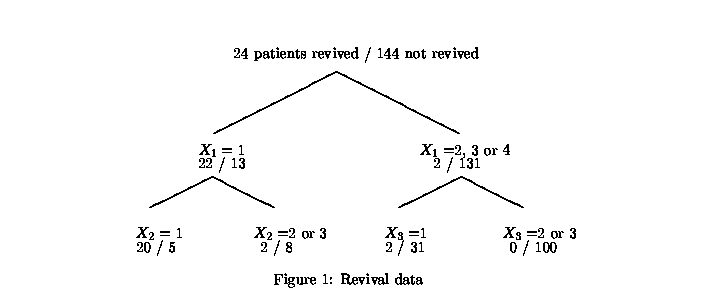
\includegraphics[width=7.0in]{RPart.jpg}

So, if for example a patient has $X^{(1)}=1$ and $X^{(2)} = 3$, we would
guess him to be revivable.

CART is a boundary method, as SVM is.  Say for instance we have two
variables, represented graphically by s and t, and our root node rule is
$s > 0.62$.  In the left branch, the rule is $t > 0.8$ and in the right
branch it's $t > 0.58$.  This boils down to a boundary line as follows:

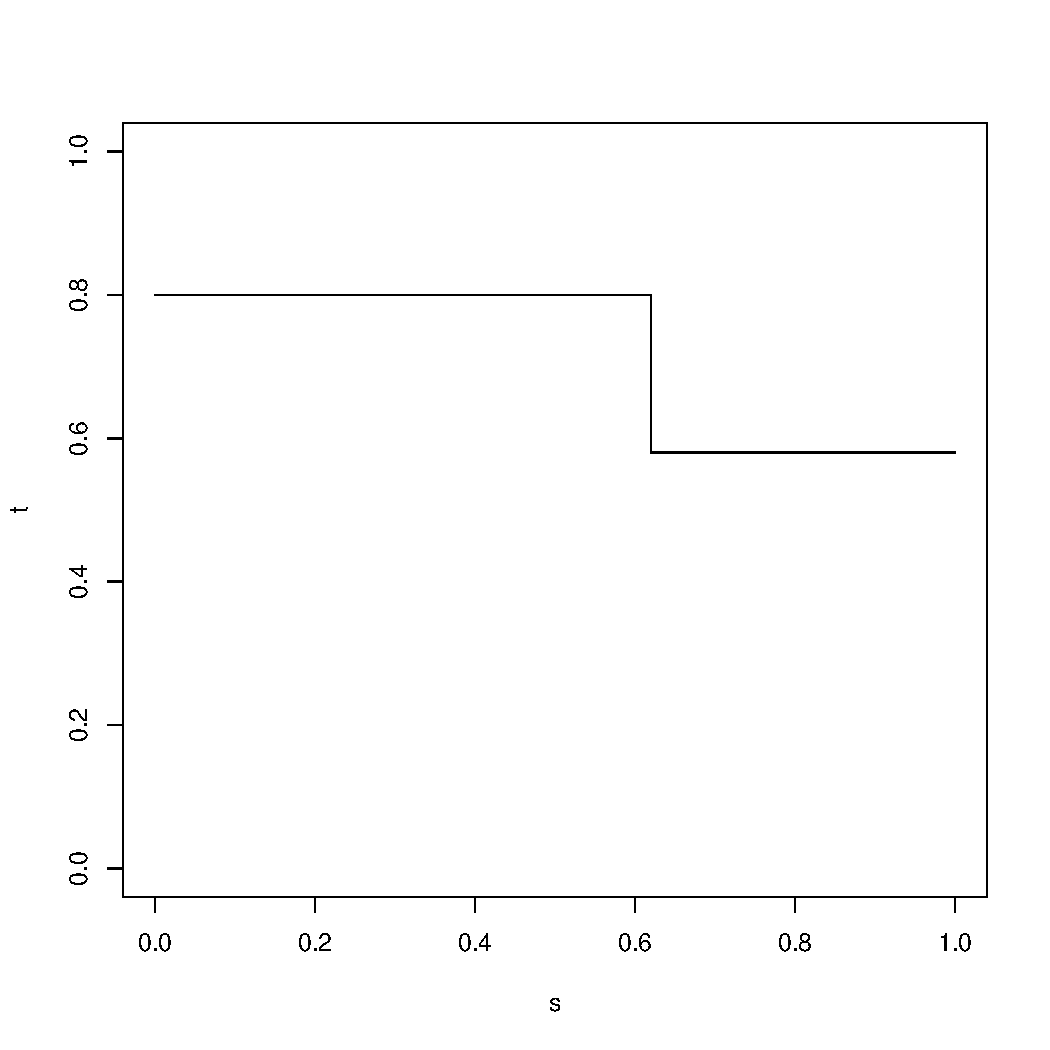
\includegraphics[width=5.0in]{CARTBound.pdf}

CART obviously has an intuitive appeal, easily explained to
nonstatisticians, and easy quite easy to implement.  It also has the
virtue of working equally well with discrete or continuous predictor
variables.

The analogs here of the h in the kernel method and k in nearest-neighbor
regression are the choice of where to define the splits, and when to stop
splitting.  Cross validation is often used for making such decisions.

\subsection{Comparison of Methods}

{\bf Beware!  There are no ``magic'' solutions to statistical problems.}
The statements one sees by some computer science researchers to the
effect that SVMs are generally superior to other prediction methods are,
unfortunately, unfounded; there just is no generally superior method.  

First, note that every one of the above methods involves some choice of
tuning parameter, such as h in the kernel method, k in the
nearest-neighbor method, the split points in CART, and in the case of
SVM, the form of kernel to use.  For SVM the choice of kernel is
crucial, yet difficult.

Second, the comparisons are often unfair, notably comparisons of the
logit model to SVM.  Such comparisons usually limit the logit
experiments to first-degree terms without interactions.  But the kernel
in SVM is essentially analogous to throwing in second-degree and
interaction terms, and so oni, (\ref{logit2}) for the logit case, thus
producing a curved partitioning line just like SVM does.

I highly recommend the site \url{www.dtreg.com/benchmarks.htm}, which
compares six different types of classification function
estimators---including logistic regression and SVM---on several dozen
real data sets.  The overall percent misclassification rates, averaged
over all the data sets, was fairly close, ranging from a high of 25.3\%
to a low of 19.2\%.  The much-vaunted SVM came in at an overall score
across all data sets of 20.3\%.  That's nice, but it was only a tad
better than logit's 20.9\%---and remember, that's with logit running
under the handicap of having only first-degree terms.

Or consider the annual KDDCup competition, in which teams from around
the world compete to solve a given classification problem with the
lowest misclassification rate.  In KDDCup2009, for instance, none of the
top teams used SVM.  See {\it SIGKDD Explorations}, December 2009 issue.

Considering that logit has a big advantage in that one gets an actual
equation for the classification function, complete with parameters which
we can estimate and make confidence intervals for, it is not clear just
what role SVM and the other nonparametric estimators should play, in
general, though in specific applications they may be appropriate.

\section{Symmetric Relations Among Several Variables}

{\it It is a very sad thing that nowadays there is so little useless
information}---Oscar Wilde, famous 19th century writer

Unlike the case of regression analysis, where the response/dependent
variable plays a central role, we are now interested in symmetric
relations among several variables.  Often our goal is {\bf dimension
reduction}, meaning compressing our data into just a few important
variables.

Dimension reduction ties in to the Oscar Wilde quote above, which is a
complaint that there is too {\it much} information of the use{\it ful}
variety.  We are concerned here with reducing the complexity of that
information to a more manageable, simple set of variables.

Here we cover two of the most widely-used methods, {\bf principal
components analysis} for continuous variables, and the {\bf log-linear model}
for the discrete case.

\subsection{Principal Components Analysis}
\label{pca}

Consider a random vector $X = (X_1,X_2)'$.  Suppose the two
components of X are highly correlated with each other.  
Then for some constants c and d,

\begin{equation}
\label{onedim}
X_2 \approx c + d X_1
\end{equation}

Then in a sense there is really just one random variable here, as the
second is nearly equal to some linear combination of the first.  The
second provides us with almost no new information, once we have the
first.

In other words, even though the vector X roams in two-dimensional space,
it usually sticks close to a one-dimensional object, namely the line
(\ref{onedim}).  We saw a graph illustrating this in our chapter on
multivariate distributions, page \pageref{rho2}.

In general, consider a k-component random vector 

\begin{equation}
X = (X_1,...,X_k)'
\end{equation}

We again wish to investigate whether just a few, say w, of the $X_i$ tell
almost the whole story, i.e. whether most $X_j$ can be expressed
approximately as linear combinations of these few $X_i$.  In other
words, even though X is k-dimensional, it tends to stick close to some
w-dimensional subspace.

Note that although (\ref{onedim}) is phrased in prediction terms, we are
not (or more accurately, not necessarily) interested in prediction here.
We have not designated one of the $X^{(i)}$ to be a response variable
and the rest to be predictors.

Once again, the Principle of Parsimony is key.  If we have, say, 20 or
30 variables, it would be nice if we could reduce that to, for example,
three or four.  This may be easier to understand and work with, albeit
with the complication that our new variables would be linear
combinations of the old ones.

\subsection{How to Calculate Them}

Here's how it works.  The theory of linear algebra says that since $\Sigma$
is a symmetric matrix, it is diagonalizable, i.e. there is a real matrix Q
for which 

\begin{equation}
\label{qsigq}
Q' \Sigma Q = D
\end{equation}

where D is a diagonal matrix.  (This is a special case of {\bf singular
value decomposition}.) The columns $C_i$ of Q are the eigenvectors of
$\Sigma$, and it turns out that they are orthogonal to each other, i.e.
their dot product is 0.

Let 

\begin{equation}
W_i = C_i'X, ~ i = 1,...,k
\end{equation}

so that the $W_i$ are scalar random variables, and set 

\begin{equation}
W = (W_1,...,W_k)'
\end{equation}

Then

\begin{equation}
W = Q' X
\end{equation}

Now, use the material on covariance matrices from our chapter on
multivariate analysis, page \pageref{covawaprime},

\begin{equation}
Cov(W) = Cov(Q'X) = Q' Cov(X) Q = D ~~ \textrm{(from (\ref{qsigq}))}
\end{equation}

Note too that if X has a multivariate normal distribution (which we are
not assuming), then W does too.

Let's recap:

\begin{itemize}

\item We have created new random variables $W_i$ as linear combinations
of our original $X_j$.

\item The $W_i$ are uncorrelated.  Thus if in addition X has a
multivariate normal distribution, so that W does too, then the $W_i$
will be independent.

\item The variance of $W_i$ is given by the i$^{th}$ diagonal element of
D.

\end{itemize}

The $W_i$ are called the {\bf principal components} of the distribution
of X.

It is customary to relabel the $W_i$ so that $W_1$ has the largest
variance, $W_2$ has the second-largest, and so on.  We then choose those
$W_i$ that have the larger variances, and discard the others, because
the latter, having small variances, are close to constant and thus carry
no information.  

All this will become clearer in the example below.

\subsection{Example:  Forest Cover Data}

Let's try using principal component analysis on the forest cover data
set we've looked at before.  There are 10 continuous variables (also
many discrete ones, but there is another tool for that case, the
log-linear model, discussed in Section \ref{loglin}).

In my R run, the data set (not restricted to just two forest cover
types, but consisting only of the first 1000 observations) was in the
object {\bf f}.  Here are the call and the results:

\begin{Verbatim}[fontsize=\relsize{-2}]
> prc <- prcomp(f[,1:10])
> summary(prc)
Importance of components:
                            PC1      PC2      PC3      PC4      PC5 PC6
Standard deviation     1812.394 1613.287 1.89e+02 1.10e+02 96.93455 30.16789
Proportion of Variance    0.552    0.438 6.01e-03 2.04e-03  0.00158 0.00015
Cumulative Proportion     0.552    0.990 9.96e-01 9.98e-01  0.99968 0.99984
                            PC7      PC8 PC9  PC10
Standard deviation     25.95478 16.78595 4.2 0.783
Proportion of Variance  0.00011  0.00005 0.0 0.000
Cumulative Proportion   0.99995  1.00000 1.0 1.000
\end{Verbatim}

You can see from the variance values here that R has scaled the $W_i$ so
that their variances sum to 1.0.  (It has not done so for the standard
deviations, which are for the nonscaled variables.) This is fine, as we
are only interested in the variances relative to each other, i.e. saving
the principal components with the larger variances.

What we see here is that eight of the 10 principal components have very
small variances, i.e. are close to constant.  In other words, though we
have 10 variables $X_1,...,X_{10}$, there is really only two
variables' worth of information carried in them.  

So for example if we wish to predict forest cover type from these 10
variables, we should only use two of them.  We could use $W_1$ and
$W_2$, but for the sake of interpretability we stick to the original X
vector; we can use any two of the $X_i$.

The coefficients of the linear combinations which produce W from X, i.e.
the Q matrix, are available via {\bf prc\$rotation}.

\subsection{Log-Linear Models}
\label{loglin}

Here we discuss a procedure which is something of an analog of principal
components for discrete variables.  Our material on ANOVA will also come
into play.  It is recommended that the reader review Sections \ref{anova}
and \ref{pca} before continuing.

\subsubsection{The Setting}

Let's consider a variation on the software engineering example in
Sections \ref{examples} and \ref{anova}.  Assume we have the factors,
IDE, Language and Education.  Our change---{\bf of extreme
importance}---is that we will now assume that these factors are {\bf
RANDOM}.  What does this mean?

In the original example described in Section \ref{examples}, programmers
were {\it assigned} to languages, and in our extensions of that example,
we continued to assume this.  Thus for example the number of programmers
who use an IDE and program in Java was fixed; if we repeated the
experiment, that number would stay the same.  If we were sampling from
some programmer population, our new sample would have new programmers,
but the number using and IDE and Java would be the same as before, as
our study procedure specifies this.

By contrast, let's now assume that we simply sample programmers at
random, and ask them whether they prefer to use an IDE or not, and which
language they prefer.\footnote{Other sampling schemes are possible too.}
Then for example the number of programmers who prefer to use an IDE and
program in Java will be random, not fixed; if we repeat the experiment,
we will get a different count.

Suppose we now wish to investigate relations between the factors.
Are choice of platform and language related to education, for instance?

\subsubsection{The Data}

Denote our three factors by $X^{(s)}$, s = 1,2,3.  Here $X^{(1)}$, IDE,
will take on the values 1 and 2 instead of 1 and 0 as before, 1 meaning
that the programmer prefers to use an IDE, and 2 meaning not so.
$X^{(3)}$ changes this way too, and $X^{(2)}$ will take on the values 1
for C++, 2 for Java and 3 for C.  Note that we no longer use indicator
variables.

Let $X_r^{(s)}$ denote the value of $X^{(s)}$ for the r$^{th}$
programmer in our sample, r = 1,2,...,n.  Our data are the counts

\begin{equation}
N_{ijk} = \textrm{number of r such that } X_r^{(1)} = i, X_r^{(2)} = j
\textrm{ and } X_r^{(3)} = k
\end{equation}

For instance, if we sample 100 programmers, our data might look like
this:

\begin{Verbatim}[fontsize=\relsize{-2}]
prefers to use IDE:

                   Bachelor's or less     Master's or more
           C++                     18                   15
          Java                     22                   10
             C                      6                    4
\end{Verbatim}

\begin{Verbatim}[fontsize=\relsize{-2}]
prefers not to use IDE:

                   Bachelor's or less     Master's or more
           C++                      7                    4
          Java                      6                    2
             C                      3                    3
\end{Verbatim}

So for example $N_{122} = 10$ and $N_{212} = 4$.

Here we have a three-dimensional {\bf contingency table}.  Each $N_{ijk}$
value is a {\bf cell} in the table.

\subsubsection{The Models}

Let $p_{ijk}$ be the population probability of a randomly-chosen
programmer falling into cell ijk, i.e.

\begin{equation}
p_{ijk} 
= P \left ( X^{(1)} = i \textrm{ and } X^{(2)} = j \textrm{ and } X^{(3)} = k \right ) 
= E(N_{ijk}) / n
\end{equation}

As mentioned, we are interested in relations between the factors, in the
form of independence, full and partial.  Consider first the
case of full independence:

\begin{eqnarray}
p_{ijk} &=&
P \left ( X^{(1)} = i \textrm{ and } X^{(2)} = j \textrm{ and } X^{(3)} = k \right ) \\ 
&=& P \left ( X^{(1)} = i \right )
\cdot P \left ( X^{(2)} = j \right )
\cdot P \left ( X^{(3)} = k \right ) 
\label{fullind}
\end{eqnarray}

Taking logs of both sides in (\ref{fullind}), we see that independence
of the three factors is equivalent to saying 

\begin{equation}
\label{abc}
\log(p_{ijk}) = a_i + b_j + c_k
\end{equation}

for some numbers $a_i$, $b_j$ and $c_j$.  The numbers must be
nonpositive, and since

\begin{equation}
\sum_{m} P(X^{(s)} = m) = 1
\end{equation}

we must have, for instance,

\begin{equation}
\label{sum1}
\sum_{g=1}^2 \exp(c_g) = 1
\end{equation}

The point is that (\ref{abc}) looks like our no-interaction ANOVA
models, e.g. (\ref{nointeraction}).  On the other hand, if we assume
instead that Education is independent of IDE and Language but that IDE
and Language are not independent of each other, our model would be

\begin{eqnarray}
\log(p_{ijk}) &=& 
P \left ( X^{(1)} = i \textrm{ and } X^{(2)} = j \right )
\cdot P \left ( X^{(3)} = k \right ) \\
&=& a_i + b_j + d_{ij} + c_k \label{semiindep}
\end{eqnarray}

Here we have written $P \left ( X^{(1)} = i \textrm{ and } X^{(2)} =
j \right )$ as a sum of ``main effects'' $a_i$ and $b_j$, and
``interaction effects,'' $d_{ij}$, analogous to ANOVA.  

Another possible model would have IDE and Language conditionally
independent, given Education, meaning that at any level of education, a
programmer's preference to use IDE or not, and his choice of programming
language, are not related.  We'd write the model this way:

\begin{eqnarray}
\log(p_{ijk}) &=& 
P \left ( X^{(1)} = i \textrm{ and } X^{(2)} = j \right )
\cdot P \left ( X^{(3)} = k \right ) \\
&=& a_i + b_j + f_{ik} + h_{jk} + c_k \label{semiindep2}
\end{eqnarray}

Note carefully that the type of independence in (\ref{semiindep2}) has a
quite different interpretation than that in (\ref{semiindep}).

The full model, with no independence assumptions at all, would have
three two-way interaction terms, as well as a three-way interaction term.

\subsubsection{Parameter Estimation}

Remember, whenever we have parametric models, the statistician's ``Swiss
army knife'' is maximum likelihood estimation.  That is what is most
often used in the case of log-linear models.

How, then, do we compute the likelihood of our data, the $N_{ijk}$?
It's actually quite straightforward, because the $N_{ijk}$ have a
multinomial distribution.  Then 

\begin{equation}
\label{like}
L =
\frac
{n!}
{\Pi_{i,j,k} N_{ijk}!}
p_{ijk}^{N_{ijk}}
\end{equation}

We then write the $p_{ijk}$ in terms of our model parameters.
Take for example (\ref{semiindep}), where we write

\begin{equation}
\label{xxx}
p_{ijk} 
= e^{a_i + b_j + d_{ij} + c_k} 
\end{equation}

We then substitute (\ref{xxx}) in (\ref{like}), and maximize the latter
with respect to the $a_i$, $b_j$, $d_{ij}$ and $c_k$, subject to
constraints such as (\ref{sum1}).

The maximization may be messy.  But certain cases have been worked out
in closed form, and in any case today one would typically do the
computation by computer.  In R, for example, there is the {\bf loglin()}
function for this purpose.

\subsubsection{The Goal:  Parsimony Again}

Again, we'd like ``the simplest model possible, but not simpler.''  This 
means a model with as much independence between factors as possible,
subject to the model being accurate.

Classical log-linear model procedures do model selection by hypothesis
testing, testing whether various interaction terms are 0.  The tests
often parallel ANOVA testing, with chi-square distributions arising
instead of F-distributions.

\section{Simpson's (Non-)Paradox}

Suppose each individual in a population either possesses or does not
possess traits {\it A}, {\it  B} and {\it C}, and that we wish to
predict trait {\it A}.  Let $\bar{A}$, $\bar{B}$ and $\bar{C}$ denote
the situations in which the individual does not possess the given trait.
Simpson's Paradox then describes a situation in which

\begin{equation}
P(A|B) > P(A|\bar{B})
\end{equation}

\noindent and yet

\begin{equation}
P(A|B,C) < P(A|\bar{B},C)
\end{equation}

In other words, the possession of trait $B$ seems to have a positive
predictive power for $A$ by itself, but when in addition trait $C$ is
held constant, the relation between $B$ and $A$ turns negative.

An example is given by Fabris and Freitas,\footnote{C.C. Fabris and A.A.
Freitas. Discovering Surprising Patterns by Detecting Occurrences of
Simpson's Paradox.  In {\it Research and Development in Intelligent
Systems XVI (Proc. ES99, The 19th SGES Int. Conf. on Knowledge-Based
Systems  and  Applied Artificial Intelligence)}, 148-160.
Springer-Verlag, 1999 } concerning a classic study of tuberculosis
mortality in 1910.  Here the attribute $A$ is mortality, $B$ is city
(Richmond, with $\bar{B}$ being New York), and $C$ is race
(African-American, with $\bar{C}$ being Caucasian).  In probability
terms, the data show that (these of course are sample
estimates)

\begin{itemize}

\item P(mortality $|$ Richmond) = 0.0022

\item P(mortality $|$ New York) = 0.0019

\item P(mortality $|$ Richmond, black) = 0.0033

\item P(mortality $|$ New York, black) = 0.0056

\item P(mortality $|$ Richmond, white) = 0.0016

\item P(mortality $|$ New York, white) = 0.0018

\end{itemize}

\noindent The data also show that

\begin{itemize}

\item P(black $|$ Richmond) = 0.37

\item P(black $|$ New York) = 0.002

\end{itemize}

\noindent a point which will become relevant below.

At first, New York looks like it did a better job than Richmond.
However, once one accounts for race, we find that New York is actually
worse than Richmond.  Why the reversal?  The answer stems from the fact
that racial inequities being what they were at the time, blacks with the
disease fared much worse than whites.  Richmond's population was 37\%
black, proportionally far more than New York's 0.2\%.  So, Richmond's
heavy concentration of blacks made its overall mortality rate look worse
than New York's, even though things were actually much worse in New
York.

But is this really a ``paradox''?   Closer consideration of this example
reveals that the only reason this example (and others like it) is
surprising is that the predictors were used in the wrong order.  One
normally looks for predictors one at a time, first finding the best
single predictor, then the best pair of predictors, and so on.  If this
were done on the above data set, the first predictor variable chosen
would be race, not city.  In other words, the sequence of analysis would
look something like this: 

\begin{itemize}

\item P(mortality $|$ black) = 0.0048

\item P(mortality $|$ white) = 0.0018

\item P(mortality $|$ black, Richmond) = 0.0033

\item P(mortality $|$ black, New York) = 0.0056

\item P(mortality $|$ white, Richmond) = 0.0016

\item P(mortality $|$ white, New York) = 0.0018

\end{itemize}

The analyst would have seen that race is a better predictor than city,
and thus would have chosen race as the best single predictor.  The
analyst would then investigate the race/city predictor pair, and
would never reach a point in which city alone were in the
selected predictor set.  Thus no anomalies would arise.

\startproblemset

\oneproblem
Suppose we are interested in documents of a certain type, which we'll
call Type 1.  Everything that is not Type 1 we'll call Type 2, with
a proportion $q$ of all documents being Type 1.  Our goal will be to 
try to guess document type by the presence of absence of a certain word;
we will guess Type 1 if the word is present, and otherwise will guess
Type 2.  

Let $T$ denote document type, and let $W$ denote the event that the word
is in the document.  Also, let $p_i$ be the proportion of documents that
contain the word, among all documents of Type i, i = 1,2.  The event $C$
will denote our guessing correctly.

Find the overall probability of correct classification, $P(C)$, and also
$P(C | W)$.

Hint:  Be careful of your conditional and unconditional probabilities
here.

\oneproblem
We showed that (\ref{oneonelogodds2}) reduces to the logistic model in
the case in which the distribution of $X$ given $Y$ is normal.  Show
that this is also true in the case in which that distribution is
exponential, i.e.

\begin{equation}
f_{X|Y}(t,i) = \lambda_i e^{-\lambda_i t}, ~ t > 0
\end{equation}

% \section{Linear Regression with All Predictors Being Nominal Variables:
% Analysis of ``Variance''}
% \label{anova}
% 
% (Note to readers:  The material in this section is arguably of lesser
% value to computer science.  As such, it can easily be skipped.  However,
% it does provide motivation for our treatment of the log-linear model in
% Section \ref{loglin}.)
% 
% Continuing the ideas in Section \ref{nominal}, suppose in the software
% engineering study they had kept the project size constant, and instead
% of $X^{(1)}$ being project size, this variable recorded whether the
% programmer uses an integrated development environment (IDE).  Say
% $X^{(1)}$ is 1 or 0, depending on whether the programmer uses the
% Eclipse IDE or no IDE, respectively.  Continue to assume the study
% included the nominal Language variable, i.e. assume the study included
% the indicator variables $X^{(2)}$ (C++) and $X^{(3)}$ (Java).  Now all
% of our predictors would be nominal/indicator variables.  Regression
% analysis in such settings is called {\bf analysis of variance} (ANOVA).
% 
% Each nominal variable is called a {\bf factor}.  So, in our software
% engineering example, the factors are IDE and Language.  Note again that
% in terms of the actual predictor variables, each factor is represented
% by one or more indicator variables; here IDE has one indicator variables
% and Language has two.
% 
% Analysis of variance is a classic statistical procedure, used heavily in
% agriculture, for example.  We will not go into details here, but mention
% it briefly both for the sake of completeness and for its relevance to
% Sections \ref{interaction} and \ref{loglin}.  (The reader is strongly
% advised to review Sections \ref{interaction} before continuing.)
% 
% \subsection{It's a Regression!}
% 
% The term {\it analyisis of variance} is a misnomer.  A more appropriate
% name would be {\bf analysis of means}, as it is in fact a regression
% analysis, as follows.
% 
% First, note in our software engineering example we basically are talking
% about six groups, because there are six different combinations of values
% for the triple $(X^{(1)},X^{(2)},X^{(3)})$.  For instance, the triple
% (1,0,1) means that the programmer is using an IDE and programming in
% Java.  Note that triples of the form (w,1,1) are impossible.
% 
% So, all that is happening here is that we have six groups with six
% means.  But that is a regression!  Remember, for variables U and V,
% $m_{V;U}(t)$ is the mean of all values of V in the subpopulation group
% of people (or cars or whatever) defined by U = s.  If U is a continuous
% variable, then we have infinitely many such groups, thus infinitely many
% means.  In our software engineering example, we only have six groups,
% but the principle is the same.  We can thus cast the problem in
% regression terms:
% 
% \begin{equation}
% m_{Y;X}(i,j,k) = E(Y|X^{(1)}=i, X^{(2)}=j, X^{(3)}=k), ~ i,j,k=0,1, j+k
% \leq 1
% \end{equation}
% 
% Note the restriction $j+k \leq 1$, which reflects the fact that j and k
% can't both be 1.
% 
% Again, keep in mind that we are working with means.  For instance,
% $m_{Y;X}(0,1,0)$ is the population mean project completion time for
% the programmers who do not use Eclipse and who program in C++.
% 
% Since the triple (i,j,k) can take on only six values, m can be modeled
% fully generally in the following six-parameter linear form:
% 
% \begin{equation}
% \label{full}
% m_{Y;X}(i,j,k) = \beta_0 + \beta_1 i + \beta_2 j + \beta_3 k
% + \beta_4 ij
% + \beta_5 ik
% \end{equation}
% 
% where $\beta_4$ and $\beta_5$ are the coefficients of two interaction
% terms, as in Section \ref{interaction}.  
% 
% \subsection{Interaction Terms}
% 
% It is crucial to understand the interaction terms.  Without the ij and
% ik terms, for instance, our model would be
% 
% \begin{equation}
% \label{nointeraction}
% m_{Y;X}(i,j,k) = \beta_0 + \beta_1 i + \beta_2 j + \beta_3 k
% \end{equation}
% 
% which would mean (as in Section \ref{interaction}) that the difference
% between using Eclipse and no IDE is the same for all three programming
% languages, C++, Java and C.  That common difference would be $\beta_1$.
% If this condition---the impact of using an IDE is the same across
% languages---doesn't hold, at least approximately, then we would use the
% full model, (\ref{full}).  More on this below.
% 
% Note carefully that there is no interaction term corresponding to jk,
% since that quantity is 0, and thus there is no three-way interaction
% term corresponding to ijk either.  
% 
% But suppose we add a third factor, Education, represented by the
% indicator $X^{(4)}$, having the value 1 if the programmer has a least a
% Master's degree, 0 otherwise.  Then m would take on 12 values, and the
% full model would have 12 parameters: 
% 
% \begin{equation}
% \label{full3}
% m_{Y;X}(i,j,k,l) = \beta_0 + \beta_1 i + \beta_2 j + \beta_3 k + \beta_4 l
% + \beta_5 ij
% + \beta_6 ik
% + \beta_7 il
% + \beta_8 jl
% + \beta_9 kl
% + \beta_{10} ijl
% + \beta_{11} ikl
% \end{equation}
% 
% Again, there would be no ijkl term, as jk = 0.
% 
% Here $\beta_1$, $\beta_2$, $\beta_3$ and $\beta_4$ are called the {\bf
% main effects}, as opposed to the coefficients of the interaction terms,
% called of course the {\bf interaction effects}.
% 
% The no-interaction version would be
% 
% \begin{equation}
% \label{noint3}
% m_{Y;X}(i,j,k,l) = \beta_0 + \beta_1 i + \beta_2 j + \beta_3 k + \beta_4 l
% \end{equation}
% 
% \subsection{Now Consider Parsimony}
% 
% In the three-factor example above, we have 12 groups and 12 means.  Why
% not just treat it that way, instead of applying the powerful tool of
% regression analysis?  The answer lies in our desire for parsimony, as
% noted in Section \ref{overfit}.
% 
% If for example (\ref{noint3}) were to hold, at least approximately, we
% would have a far more satisfying model.  We could for instance then talk
% of ``the'' effect of using an IDE, rather than qualifying such a
% statement by stating what the effect would be for each different
% language and education level.  Moreover, if our sample size is not very
% large, we would get more accurate estimates of the various subpopulation
% means, once again due to bias/variance tradeoff.
% 
% Or it could be that, while (\ref{noint3}) doesn't hold, a model with only
% two-way interactions,
% 
% \begin{equation}
% \label{2way}
% m_{Y;X}(i,j,k,l) = \beta_0 + \beta_1 i + \beta_2 j + \beta_3 k + \beta_4 l
% + \beta_5 ij
% + \beta_6 ik
% + \beta_7 il
% + \beta_8 jl
% + \beta_9 kl
% \end{equation}
% 
% does work well.  This would not be as nice as (\ref{noint3}), but it
% still would be more parsimonious than (\ref{full3}).
% 
% Accordingly, the major thrust of ANOVA is to decide how rich a model is
% needed to do a good job of describing the situation under study.  There
% is an implied hierarchy of models of interest here:
% 
% \begin{itemize}
% 
% \item the full model, including two- and three-way interactions,
% (\ref{full3})
% 
% \item the model with two-factor interactions only, (\ref{2way})
% 
% \item the no-interaction model, (\ref{noint3})
% 
% \end{itemize}
% 
% Traditionally these are determined via hypothesis testing, which
% involves certain partitionings of sums of squares similar to
% (\ref{sumsq}).  (This is where the name {\it analysis of variance} stems
% from.)  The null distribution of the test statistic often turns out to
% be an F-distribution.  Of course, in this book, we consider hypothesis
% testing inappropriate, preferring to give some careful thought to the
% estimated parameters, but it is standard.  Further testing can be done
% on individual $\beta_1$ and so on.  Often people use simultaneous
% inference procedures, discussed briefly in Section \ref{simultancis} of
% our chapter on estimation and testing, since many tests are performed.
% 
% \subsection{Reparameterization}
% 
% Classical ANOVA uses a somewhat different parameterization than that
% we've considered here.  For instance, consider a single-factor setting
% (called {\bf one-way ANOVA}) with three levels.  Our predictors are then
% $X^{(1)}$ and $X^{(2)}$.  Taking our approach here, we would write
% 
% \begin{equation}
% m_{Y;X}(i,j) = \beta_0 + \beta_1 i + \beta_2 j 
% \end{equation}
% 
% The traditional formulation would be
% 
% \begin{equation}
% \mu_i = \mu + \alpha_i, ~ i = 1,2,3
% \end{equation}
% 
% where
% 
% \begin{equation}
% \mu = \frac{\mu_1+\mu_2+\mu_3}{3}
% \end{equation}
% 
% and 
% 
% \begin{equation}
% \alpha_i = \mu_i - \mu
% \end{equation}
% 
% Of course, the two formulations are equivalent.  It is left to the
% reader to check that, for instance, 
% 
% \begin{equation}
% \mu = \beta_0 + \frac{\beta_1+\beta_2}{2}
% \end{equation}
% 
% There are similar formulations for ANOVA designs with more than one
% factor.
% 
% Note that the classical formulation overparameterizes the problem.  In
% the one-way example above, for instance, there are four parameters
% ($\mu$, $\alpha_1$, $\alpha_2$, $\alpha_3$) but only three groups.
% This would make the system indeterminate, but we add the constraint
% 
% \begin{equation}
% \sum_{i=1}^3 \alpha_i = 0
% \end{equation}
% 
% Equation (\ref{betahat}) then must make use of {\bf generalized matrix
% inverses}.
% 
% \section{Clustering}
% 
% HERE ONE **REALLY* HAS TROUBLE 
% WITH "WHAT DOES IT MEAN?:

% pdf("CARTBound.pdf")
% plot(c(0,1),c(0,1),type="n",xlab="s",ylab="t")
% lines(c(0,0.62),c(0.8,0.8))
% lines(c(0.62,1),c(0.58,0.58))
% lines(c(0.62,0.62),c(0.58,0.8))
% dev.off()
% 
% 
% lines(c(0.62,0.62),c(0,1))

